\section{Modeling Mutation}\label{sec:mm}
In this section, we describe our proposed 3-parameter $\theta = \{ d, u, c\}$ mutation model.

\subsection{Repeat Unit Change Per Generation}\label{subsec:rucpg}
TODO: (1) Mention the stepwise mutation model, (2) Mention the two-phase model,
(3) We are going with the stepwise mutation model.

\subsection{Mutation Rate Dependence on Repeat Unit}\label{subsec:mrdonru}
TODO: (1) Mention the rate equality, (2) Mention the repeat length dependence on repeat unit,
(3) We are going with the repeat length dependence.

\subsection{Presence of Mutational Bias}\label{subsec:pomb}
TODO: (1) Mention the requirement of repeat length dependence, (2) Mention the constant bias parameter,
(3) Mention the linear bias, (4) Mention the focal bias

Our focal bias $\hat{\ell} $is defined as the point where $\mu_u$ and $\mu_d$ intersect:
\begin{equation}
    \hat{\ell} = \frac{-c}{\frac{d}{u} - d}
%    \begin{aligned}
%        \mu_u &= \mu_d \\
%        \frac{d}{u}\ell + c &= d\ell \\
%        (\frac{d}{u} - d)\ell &= -c \\
%        \ell &= \frac{-c}{\frac{d}{u} - d}
%    \end{aligned}
\end{equation}

\begin{figure}
    \centering{\pgfplotsset{compat=1.5}
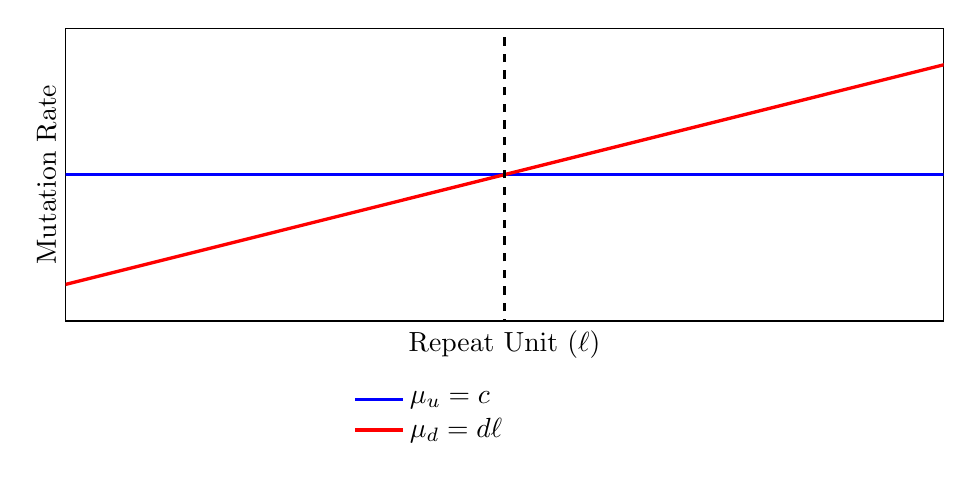
\begin{tikzpicture}
    \begin{axis}[
    width=1.05\linewidth, height=5.3cm,
    ylabel={Mutation Rate}, ymin=0.01, ymax=0.05,
    xlabel={Repeat Unit ($\ell$)}, xmin=6, xmax=18,
    xtick={0, 2, 4, 6, 8, 10, 12, 14, 16, 18, 20, 22, 24},
    samples=100, no markers, enlargelimits=false, legend style={at={(0.5,-0.2)},anchor=north,draw=none},
    legend cell align={left}, domain=0:25, ticks=none
    ]
        \addplot+[very thick]{0.03};
        \addlegendentry{$\mu_u = c$};

        \addplot+[very thick] {0.0025*x};
        \addlegendentry{\vspace*{5em}$\mu_d = d\ell$ \hspace*{5em}};

        \addplot+[very thick, black, dashed, forget plot] coordinates {(12, 0) (12, 0.05)};
    \end{axis}
\end{tikzpicture}}
    \caption{Our mutation model for $d=0.0025, u=1.2, c=0.005$.
    Our focal bias with these parameters is $\hat{\ell}=12$.}\label{fig:mutationModel}
\end{figure}